\documentclass[12pt]{article}


\oddsidemargin .2 in
\evensidemargin .2 in
\topmargin 0 in
\textwidth 6.1 in
\textheight 8.3 in

\usepackage{float}
\usepackage{fullpage,amssymb}
\usepackage{graphicx}
\usepackage{amsmath}
\usepackage{bm}     
%\geometry{vmargin=0.5in} % adjusts the height of the color banner at the top

\allowdisplaybreaks

\newcommand{\m}[1]{\mathbf{\bm{#1}}}

\begin{document}

\title{Solutions to Problem 6 \\
Homework Assignment 3 \\
{\small {\bf AMS 206B, WINTER 2016 }} \\
}

\author{Prepared by: Mickey Warner and Xingchen (Joe) Yu}

\maketitle

\section*{Problem 6, HW 3}
\noindent Let $y_t=\rho y_{t-1} + \epsilon_t$, $\epsilon_t \overset{iid}\sim N(0,\sigma^2)$. This is a popular model in time series analysis known as the autoregressive model of order one or AR(1).
\bigskip

\noindent \textbf{(a)} \emph{Write down the conditional likelihood given $y_1$, i.e., $f(y_2,\ldots,y_n|y_1,\rho,\sigma^2)$.}
\bigskip

\noindent Since $y_t \sim N(\rho y_{t-1}, \sigma^2)$ depends only on the previous observation, we have
\begin{align*}
f(y_2,\ldots,y_n|y_1,\rho,\sigma^2) &= \prod_{t=2}^n (2\pi\sigma^2)^{-1/2}\exp\left\{-\frac{1}{2\sigma^2}(y_t-\rho y_{t-1})^2\right\} \\
&= (2\pi\sigma^2)^{-(n-1)/2} \exp\left\{-\frac{1}{2\sigma^2}\sum_{t=2}^n(y_t-\rho y_{t-1})^2\right\}
\end{align*}

\bigskip
\noindent \textbf{(b)} \emph{Assume a prior of the form $\pi(\rho, \sigma^2) \propto 1/\sigma^2$.}
\bigskip

\noindent \textbf{(i)} \emph{Find the joint posterior $p(\rho, \sigma^2|y_1,\ldots, y_n)$ based on the conditional likelihood.}
\bigskip

\noindent Using Bayes' formula and keeping only the terms that contain $\rho$ and $\sigma^2$, we obtain
\begin{align*}
p(\rho, \sigma^2|y_1, \ldots, y_n) &\propto f(y_2,\ldots,y_n|y_1,\rho,\sigma^2)\pi(\rho,\sigma^2|y_1) \\
&\propto f(y_2,\ldots,y_n|y_1,\rho,\sigma^2)\pi(\rho,\sigma^2) \\
&\propto (\sigma^2)^{-(n-1)/2} \exp\left\{-\frac{1}{2\sigma^2}\sum_{t=2}^n(y_t-\rho y_{t-1})^2\right\}(\sigma^2)^{-1} \\
&\propto (\sigma^2)^{-(n+1)/2} \exp\left\{-\frac{1}{2\sigma^2}\sum_{t=2}^n(y_t-\rho y_{t-1})^2\right\}
\end{align*}
\noindent We use the prior $\pi(\rho,\sigma^2)$ in place of $\pi(\rho,\sigma^2|y_1)$ since with large enough $n$, $y_1$ will contribute little. This simplification allows us to deal with the problems due to $y_1$.

\newpage

\noindent \textbf{(ii)} \emph{Find $p(\rho|\sigma^2,y_1,\ldots,y_n)$ and $p(\sigma^2|y_1,\ldots,y_n)$ based on the conditional likelihood.}
\bigskip

\noindent We remove the constants and work with only the necessary terms to obtain the kernels for each quantity.
\begin{align*}
p(\rho|\sigma^2,y_1,\ldots,y_n) &\propto p(\rho,\sigma^2|y_1,\ldots,y_n) \\
&\propto \exp\left\{-\frac{1}{2\sigma^2}\sum_{t=2}^n(y_t-\rho y_{t-1})^2\right\} \\
&\propto \exp\left\{-\frac{1}{2\sigma^2}\left(\sum_{t=2}^ny_t^2 - 2\rho\sum_{t=2}^ny_t y_{t-1}+\rho^2\sum_{t=2}^ny_{t-1}^2\right)\right\} \\
&\propto \exp\left\{-\frac{1}{2\sigma^2}\left(- 2\rho\sum_{t=2}^ny_t y_{t-1}+\rho^2\sum_{t=2}^ny_{t-1}^2\right)\right\} \\
&\propto \exp\left\{-\frac{\sum_{t=2}^ny_{t-1}^2}{2\sigma^2}\left(\rho^2 - 2\rho\frac{\sum_{t=2}^ny_t y_{t-1}}{\sum_{t=2}^ny_{t-1}^2}\right)\right\} \\
&\propto \exp\left\{-\frac{1}{2\frac{\sigma^2}{\sum_{t=2}^ny_{t-1}^2}}\left[\rho^2 - 2\rho\frac{\sum_{t=2}^ny_t y_{t-1}}{\sum_{t=2}^ny_{t-1}^2} + \left(\frac{\sum_{t=2}^ny_t y_{t-1}}{\sum_{t=2}^ny_{t-1}^2}\right)^2\right]\right\} \\
&\propto \exp\left\{-\frac{1}{2\frac{\sigma^2}{\sum_{t=2}^ny_{t-1}^2}}\left(\rho - \frac{\sum_{t=2}^ny_t y_{t-1}}{\sum_{t=2}^ny_{t-1}^2} \right)^2\right\}
\end{align*}

\noindent This is the kernel of a normal distribution, so we have:

\[\rho|\sigma^2,y_1,\ldots,y_2\sim N\left(\frac{\sum_{t=2}^ny_t y_{t-1}}{\sum_{t=2}^ny_{t-1}^2}, \frac{\sigma^2}{\sum_{t=2}^ny_{t-1}^2}\right) \]

\noindent To obtain $p(\sigma^2|y_1,\ldots,y_n)$ we must integrate out $\rho$ from the full posterior. The work is nothing but annoying, but like whatever. The integrand is normal kernel, equivalent to that from before, but now we have to keep the terms containing $\sigma^2$ used to complete the square.
\begin{align*}
p(\sigma^2|y_1,\ldots,y_n) &= \int p(\rho,\sigma^2|y_1,\ldots,y_n)d\rho \\
&\propto \int (\sigma^2)^{-(n+1)/2} \exp\left\{-\frac{1}{2\sigma^2}\sum_{t=2}^n(y_t-\rho y_{t-1})^2\right\} d\rho \\
&\propto (\sigma^2)^{-(n+1)/2} \int \exp\left\{-\frac{1}{2\sigma^2}\left(\sum_{t=2}^ny_t^2 - 2\rho\sum_{t=2}^ny_t y_{t-1}+\rho^2\sum_{t=2}^ny_{t-1}^2\right)\right\} d\rho \\
&\propto (\sigma^2)^{-(n+1)/2}\exp\left(-\frac{1}{2\sigma^2}\sum_{t=2}^ny_t^2\right) \times \\
& ~~~~ ~~~~ \int \exp\left\{-\frac{1}{2\sigma^2}\left(- 2\rho\sum_{t=2}^ny_t y_{t-1}+\rho^2\sum_{t=2}^ny_{t-1}^2\right)\right\} d\rho \\
&\propto (\sigma^2)^{-(n+1)/2}\exp\left(-\frac{1}{2\sigma^2}\sum_{t=2}^ny_t^2\right) \times \\
& ~~~~ ~~~~ \int \exp\left\{-\frac{\sum_{t=2}^ny_{t-1}^2}{2\sigma^2}\left(\rho^2- 2\rho\frac{\sum_{t=2}^ny_t y_{t-1}}{\sum_{t=2}^ny_{t-1}^2}\right)\right\} d\rho \\
&\propto (\sigma^2)^{-(n+1)/2}\exp\left(-\frac{1}{2\sigma^2}\sum_{t=2}^ny_t^2\right)\exp\left\{\frac{\sum_{t=2}^ny_{t-1}^2}{2\sigma^2}\cdot\left(\frac{\sum_{t=2}^ny_t y_{t-1}}{\sum_{t=2}^ny_{y-1}^2}\right)^2\right\}  \times \\
& ~~~~ ~~~~ \int \exp\left\{-\frac{\sum_{t=2}^ny_{t-1}^2}{2\sigma^2}\left[\rho^2- 2\rho\frac{\sum_{t=2}^ny_t y_{t-1}}{\sum_{t=2}^ny_{t-1}^2}+\left(\frac{\sum_{t=2}^ny_t y_{t-1}}{\sum_{t=2}^ny_{y-1}^2}\right)^2\right]\right\} d\rho \\
&\propto (\sigma^2)^{-(n+1)/2}\exp\left\{-\frac{1}{\sigma^2}\left(\frac{1}{2}\sum_{t=2}^ny_t^2 +\frac{1}{2}\frac{(\sum_{t=2}^ny_t y_{t-1})^2}{\sum_{t=2}^ny_{y-1}^2}\right)\right\}  \times \\
& ~~~~ ~~~~ \left(2\pi\frac{\sigma^2}{\sum_{t=2}^ny_{t-1}^2}\right)^{1/2} \\
&\propto (\sigma^2)^{-n/2}\exp\left\{-\frac{1}{\sigma^2}\left(\frac{1}{2}\sum_{t=2}^ny_t^2 +\frac{1}{2}\frac{(\sum_{t=2}^ny_t y_{t-1})^2}{\sum_{t=2}^ny_{y-1}^2}\right)\right\} \\
\end{align*}
\noindent We recognize this as an inverse gamma:

\[ \sigma^2|y_1,\ldots,y_n \sim IG\left(\frac{n-2}{2}, \frac{1}{2}\sum_{t=2}^ny_t^2 +\frac{1}{2}\frac{(\sum_{t=2}^ny_t y_{t-1})^2}{\sum_{t=2}^ny_{y-1}^2}\right) \]

\bigskip
\noindent \textbf{(iii)} \emph{Simulate two data sets with $n=500$ observations each. One with $\rho=0.95$, $\sigma^2=4$ and another one with $\rho=0.3$, $\sigma^2=4$. Fit the model above to the two data sets. Summarize your posterior results in both cases.}
\bigskip

\noindent We generate the two data sets using the \texttt{arima.sim()} function in \texttt{R} (code is provided in the appendix). The model is fit by obtaining posterior samples from $p(\rho,\sigma^2|y_1,\ldots,y_n)$. Since
\[ p(\rho,\sigma^2|y_1,\ldots,y_n) = p(\rho|\sigma^2,y_1,\ldots,y_n)p(\sigma^2|y_1,\ldots,y_n) \]
we can use the results from (ii). We first draw $B=10000$ (or some other large number) samples from $p(\sigma^2|y_1,\ldots,y_n)$ and then use each of these to obtain another $B$ samples from $p(\rho|\sigma^2,y_1,\ldots,y_n)$. Figure 1 and table 1 are results for the case $\rho=0.95$ and figure 2 and table 2 are for $\rho=0.30$. In each figure, we show the data as well as a density estimate of the marginal posteriors. In the tables we give the estimated mean, variance, and certain quantiles.

\begin{figure}[H]
\begin{center}
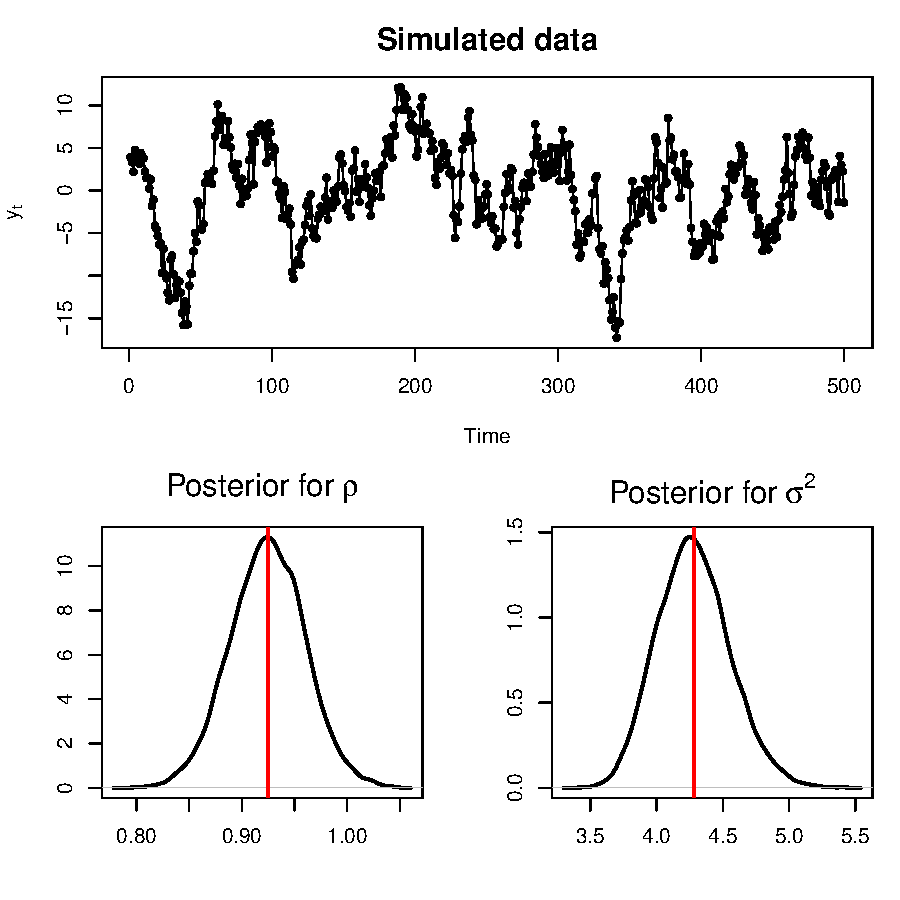
\includegraphics[scale=1.00]{figs/fig_1.pdf}
\end{center}
\caption{Top: simulated data with $n=500$, $\rho=0.95$, and $\sigma^2=4$. Bottom left: marginal posterior density of $\rho|\sigma^2,y_1,\ldots,y_2$ based on 10000 draws. Bottom right: marginal posterior density of $\sigma^2|y_1,\ldots,y_2$ based on 10000 draws. The red lines mark the means of the draws.}
\end{figure}
\bigskip

\begin{table}[H]
\begin{center}
\begin{tabular}{l|rrrrrrr}
           &  mean & var   & 0\%   & 2.5\% & 50\%  & 97.5\% & 100\% \\ \hline\hline
$\rho$     & 0.924 & 0.001 & 0.793 & 0.854 & 0.924 & 0.994  & 1.045 \\ 
$\sigma^2$ & 4.281 & 0.074 & 3.418 & 3.783 & 4.271 & 4.853  & 5.423 \\
\end{tabular}
\end{center}
\caption{Numerical summary of the posterior distributions.}
\end{table}

\newpage

\begin{figure}[H]
\begin{center}
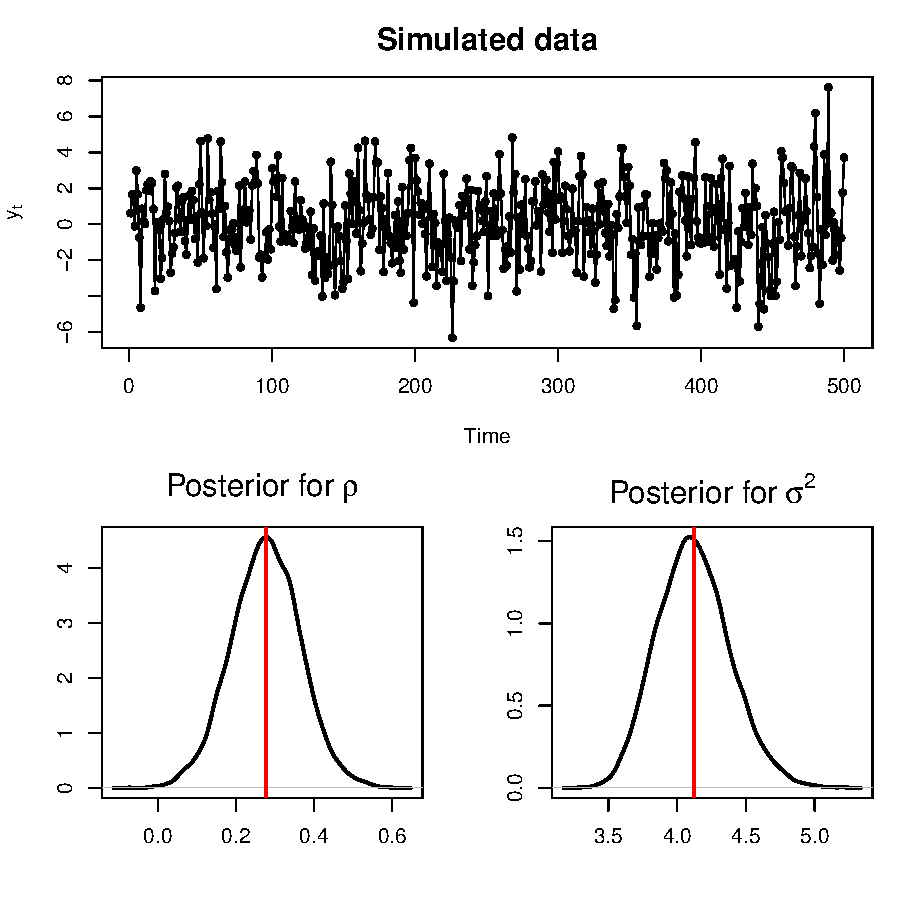
\includegraphics[scale=1.00]{figs/fig_2.pdf}
\end{center}
\caption{Top: simulated data with $n=500$, $\rho=0.30$, and $\sigma^2=4$. Bottom left: marginal posterior density of $\rho|\sigma^2,y_1,\ldots,y_2$ based on 10000 draws. Bottom right: marginal posterior density of $\sigma^2|y_1,\ldots,y_2$ based on 10000 draws. The red lines mark the means of the draws.}
\end{figure}
\bigskip

\begin{table}[H]
\begin{center}
\begin{tabular}{l|rrrrrrr}
           &  mean & var   & 0\%      & 2.5\% & 50\%  & 97.5\% & 100\% \\ \hline\hline
$\rho$     & 0.276 & 0.007 & $-0.074$ & 0.100 & 0.277 & 0.450  & 0.610 \\
$\sigma^2$ & 4.121 & 0.069 & 3.290    & 3.642 & 4.111 & 4.673  & 5.221 \\
\end{tabular}
\end{center}
\caption{Numerical summary of the posterior distributions.}
\end{table}

\newpage

\section*{Code}

\begin{footnotesize}
\begin{verbatim}
##### HW 3, Problem 6
sig = sqrt(4)
n = 500

### Generating Data
set.seed(1)
ar = 0.95
#ar = 0.30
x1 = arima.sim(list(ar=ar),n=n, sd=sig)

### Certain portions of the data vector
yn = x1[-1]
yn_1 = x1[-n]

### Sampling for sigma^2
B = 10000
alpha = (n-2)/2
beta = (sum(yn^2)-sum(yn*yn_1)^2/sum(yn_1^2))/2
po.sig = 1/rgamma(B, alpha, beta)

### Sampling for rho
mu = sum(yn*yn_1)/sum(yn_1^2)
si = po.sig/sqrt(sum(yn_1^2))
po.ro = rnorm(B, mu, si)

### Plots
#pdf("./fig_1.pdf", width = 8, height = 8)
par(mfrow=c(1,1), mar = c(4.1, 4.1, 3.1, 1.1))
layout(matrix(c(1,2,1,3),2,2))
plot(x1, type='o', pch=20, main="Simulated data", cex.main = 1.5,
    ylab = expression(y[t]))
plot(density(po.ro), main = expression("Posterior for" ~ rho),
    xlab ="", ylab="", cex.main = 1.5, lwd = 2)
abline(v = mean(po.ro), col = 'red', lwd = 2)
plot(density(po.sig), main = expression("Posterior for" ~ sigma^2),
    xlab ="", ylab="", cex.main = 1.5, lwd = 2)
abline(v = mean(po.sig), col = 'red', lwd = 2)
#dev.off()

### Summary statistics
c("mean"=mean(po.ro), "var"=var(po.ro), quantile(po.ro, c(0, 0.025, 0.5, 0.975, 1)))
c("mean"=mean(po.sig), "var"=var(po.sig), quantile(po.sig, c(0, 0.025, 0.5, 0.975, 1)))

### Scatterplot for the joint distribution
# par(mfrow=c(1,1), mar = c(5.1,4.1,4.1,2.1))
# plot(po.ro, po.sig, pch = 20, xlab="", ylab="", cex=0.5)
# mtext(expression(rho), side=1, line=3, cex=1.5)
# mtext(expression(sigma^2), side=2, line=2, cex=1.5)
\end{verbatim}
\end{footnotesize}


\end{document}
